% Full paper:
% https://github.com/pauldubois98/ESTRO2024/blob/main/full_paper.pdf
\section{Distance Between Doses}
In this section, we aim to establish a robust metric for quantifying the distance between different dose distributions.
Such a distance should provide a numerical comparison that reflects the clinical discrepancies between two dose distributions.
By developing a distance measure that captures these nuances, we can better evaluate and compare treatment plans.

\paragraph{A non-trivial task}
Quantifying the difference between two dose distributions, particularly regarding clinical impact, is inherently challenging.
This complexity arises because not all patient anatomy regions contribute equally to treatment outcomes.
Dose variations in critical structures may significantly influence clinical effects, while similar variations in less critical areas may have negligible impact.
Moreover, the potential for dose compensation (underdosing in one region counterbalancing overdosing in another) further complicates the development of a reliable metric for comparing dose distributions.
This compensatory effect is only sometimes applicable, making establishing a standardized method for assessing dose distribution clinical differences challenging.

\paragraph{Dose Evaluation}
To assess the quality of a dose distribution, dosimetrists primarily focus on DVHs as the key metric.
While they also consider aspects of the three-dimensional (3D) dose distribution, such as inter-structure dose gradients and the presence, number, and location of hot spots, their primary attention is directed towards the analysis of DVHs, which provide a comprehensive overview of dose coverage and sparing of organs at risk.

\subsection{Method}

\paragraph{Naive Doses Comparison}
The most straightforward method for comparing two dose distributions, thus defining a distance metric, is to perform a voxel-by-voxel comparison of the dose values.
However, this approach overlooks the inherent anatomical structure of the human body and the fact that not all voxels have the same clinical significance.
Consequently, even if the voxel-wise distance between two dose distributions is considerable, their overall clinical effects may still be similar.

\paragraph{Pathological example}
We constructed a simplified example, as illustrated in Figure \ref{fig:pathological_example}.
This hypothetical scenario involves a phantom model consisting of a homogeneous water-equivalent material containing a cubic planning target volume (PTV) and a cubic organ-at-risk (OAR).
Although this model lacks anatomical realism, it effectively highlights the limitations of using basic voxel-wise comparisons for dose evaluation.
It emphasizes the need for more sophisticated techniques to capture clinically relevant differences in dose distributions accurately.
\begin{figure}
	\centering
	\begin{subfigure}{0.44\linewidth}
		\includegraphics[width=\linewidth]{dose_distances_figures/example\_3d\_doses.pdf}
		\caption{3D visualization of the two doses on the phantom body.}
		\label{fig:pathological_example-3d_doses}
	\end{subfigure}
	\begin{subfigure}{0.55\linewidth}
		\includegraphics[width=\linewidth]{dose_distances_figures/example\_bixels.pdf}
		\caption{2D view of the bixels activation of the two doses.}
		\label{fig:pathological_example-bixels}
	\end{subfigure}
	\begin{subfigure}{0.75\linewidth}
		\includegraphics[width=\linewidth]{dose_distances_figures/example\_dvh.pdf}
		\caption{Dose-Volume Histograms of the two doses on the phantom body.}
		\label{fig:pathological_example-dvh}
	\end{subfigure}
	\caption{Example of two doses that have the same clinical effect (measured from the DVHs), but very different voxel-wise dose values.}
	\label{fig:pathological_example}
\end{figure}

\subsubsection{Doses Samples}
We assessed the efficacy of our proposed method for comparing radiation doses using the TG-119 Prostate case, a well-established benchmark for evaluating radiation therapy plans \cite{AAPM-TG119}.
The TG-119 dataset includes predefined dose objectives, which we utilized to formulate our cost function.
We performed optimizations with different weight assignments applied to each constraint to generate varying treatment dose distributions for the same patient case under identical constraints.

\subsubsection{Distances Between Doses}
\paragraph{Comparing Doses Voxel-wise}
When two radiation dose distributions are closely aligned, the voxel-wise comparison is an effective measure, as it can be assumed that the global distribution is similar.
This approach allows for a detailed comparison of local dose variations.
Mathematically, given the voxel-wise dose $\textbf{d}$, the distance between two dose distributions, $\textbf{d}^1$ and $\textbf{d}^2$, is defined as the norm of their difference:
$\sum_{v \in \mathcal{V}} \lvert \textbf{d}^1_v - \textbf{d}^2_v \rvert$, where $v$ represents the voxels in the set of interest $\mathcal{V}$, and $\textbf{d}^i_v$ is the dose value at voxel $v$ for dose distribution $\textbf{d}^i$
\footnote{This is often written as $\lvert \textbf{d}_1 - \textbf{d}_2 \rvert$, with the summation over voxels implied.}.
However, voxel-wise distance can become misleading if two regions of equal volume within the same anatomical structure have their dose values swapped.
In such cases, the voxel-wise difference would appear large despite the clinical equivalence of the two doses.
Furthermore, this method is limited to comparing doses within the same patient, as it requires a direct correspondence between the dose voxels in both distributions.

\paragraph{Comparing Dose Volume Histogram Curves}
We propose comparing the Dose Volume Histogram (DVH) curves.
We have one curve for each structure; we define the distances between doses for each structure, and in the end, we sum up all structures to end up with a single scalar distance between two doses.

\subparagraph{Discrete DVH Approximation}
The DVH is obtained after sorting the voxel-wise dose of the structure:
Let $\textbf{d} \left[s\right]$ bet the voxel-wise dose of the structure $s$ (therefore, a list, of length $n\left[s\right]$, the number of voxels that belong to the structure).
Let $\dot{\textbf{d}\left[s\right]}$ be the list above in descending order (i.e. $\dot{\textbf{d}\left[s\right]}_i > \dot{\textbf{d}\left[s\right]}_j$ if $0 < i < j \leq n\left[s\right ]$).
Then, the DVH of $s$ can be approximated by the continuous line composed of the segments linking the following points:
$\left( \dot{\textbf{d}\left[s\right]}_i, i/n\left[s\right] \right) \quad 0 < i \leq n\left[s\right]$.
Since we compute the dose voxel-wise, we may only have an approximation of the DVH.
However, in practice, most structures of interest have more than a hundred voxels, which makes the DVH approximation very precise.

Since we draw one curve per structure of interest, this capture some of the importance of voxel over others.
In fact, when analyzing a dose, doctors look at the dose volume (voxel-wise), but they also take a close look at the DVHs; this is an incentive that DVHs should contain meaningful information.

\subparagraph{Distance Measure}
To measure how different two DVH curves, we can imagine several techniques:
\begin{itemize}
	\item Fréchet distance (treating DVHs as curves in a 2D space)
	\item Hausdorff distance (treating DVHs as 1D manifolds in a 2D space)
	\item Wasserstein distance (treating DVHs as probability distributions)
	\item Kolmogorov-Smirnov test (treating DVHs as probability distributions)
	\item Total variation between curves (treating DVHs as functions)
\end{itemize}
We evaluated all the aforementioned distance metrics and propose to retain only the one that yields the most clinically meaningful results.

\subparagraph{Fréchet Distance}
DVH (Dose-Volume Histogram) curves can be interpreted as lines in R2R2 \footnote{In the case of voxel-wise dose approximations, they are represented as poly-lines in R2R2.}.
In this context, the Fréchet distance is a well-known metric for assessing the similarity between two curves, particularly useful for comparing poly-lines \cite{Efrat2002}.
It measures the minimum distance a particle would travel when simultaneously traversing both curves.
In this study, we apply the Fréchet distance to compare the DVH curves of two radiation dose distributions.

Formally, let $P$ and $Q$ represent the curves being compared, with $\gamma$ denoting a parametrization defined on the interval $\left[0,1\right]$.
The positions of a particle moving along curves $P$ and $Q$ at time $t$ are given by $P(\gamma(t))$ and $Q(\gamma(t))$, respectively.
The Fréchet distance is defined as:
$$d_{\text{Fréchet}}(P,Q) = \inf_{\gamma}{ \max_{t \in \left[ 0,1 \right]} d(P(\gamma(t)), Q(\gamma(t)))}$$

When applied to DVH curves, let $\mathcal{C}_A$ and $\mathcal{C}_B$ denote the discrete DVH curves of two dose distributions.
These curves consist of line segments connecting a series of points $\left\lbrace \mathcal{C}_A(i) = (d_i, v_i), \ 1 \leq i \leq n_A \right\rbrace $ and $\left\lbrace \mathcal{C}_B(j) = (\tilde{d}_j, \tilde{v}_j), \ 1 \leq j \leq n_B \right\rbrace $; where $d_i$ and $\tilde{d}_j$ denote the dose levels\footnote{Derived from $\textbf{d}$ after selecting voxels of the structure of interest, and sorting voxels.}, $v_i$ and $\tilde{v}_j$ represent the corresponding volumes, and $n_A$ and $n_B$ are the number of points forming $\mathcal{C}_A$ and $\mathcal{C}_B$\footnote{Here we are constantly comparing two DVH curves of the same structure on the same patient, so we always have $n_A = n_B$.}.

The Fréchet distance, in this case, is defined as the infimum over all possible traversal times.
Given that the curves are discrete line segments, the Fréchet distance can be expressed as:
$$d_{\text{Fréchet}}(\mathcal{C}_A, \mathcal{C}_B) = \min_{\substack{j: \llbracket 1, n_A \rrbracket \to \llbracket 1, n_B \rrbracket \\ j \nearrow \ (j \text{ increasing})}} \sum_{i=1}^{n_A} dist\left( \mathcal{C}_A(i), \mathcal{C}_B(j(i)) \right)$$
$$\text{where } dist\left( \mathcal{C}_A(i), \mathcal{C}_B(j(i)) \right) = \sqrt{(d_i-\tilde{d}_{j(i)})^2 + (v_i-\tilde{v}_{j(i)})^2}$$

Here, $j$ represents a (discrete) a parametrization, and $dist\left( \mathcal{C}_A(i), \mathcal{C}_B(j(i)) \right)$ is the distance between points $\mathcal{C}_A(i)$ and $\mathcal{C}_B(j(i))$.

One drawback of the Fréchet distance is its computational expense, particularly for structures with a large number of voxels.
To mitigate this, we applied the Ramer–Douglas–Peucker algorithm for curve simplification \cite{PRASAD2012843}.
We employed this algorithm with $\epsilon=0.05$, and after testing on a subset of DVH curves, it was found to accelerate computations by a factor of 3-5, while the calculated Fréchet distance deviated by less than 0.5\%.
This method was therefore used in the results presented below.


\subparagraph{Hausdorff Distance}
The Hausdorff distance is another commonly used metric for measuring the similarity between two curves \cite{Henrikson1999CompletenessAT}.
It is defined as the greatest of the shortest distances between any point on one curve and the closest point on the other.
Formally, let $X$ and $Y$ be two non-empty sets;
the Hausdorff distance between $X$ and $Y$, denoted $d_\text{Hausdorff}(X, Y)$, is given by:
$$d_\text{Hausdorff}(X, Y) = \sup_{x \in X}\inf_{y \in Y} {dist(x, y)}$$
where $dist(x, y)$ represents the distance between points $x$ and $y$ (typically, the Euclidean distance).

In this study, we treat DVH (Dose-Volume Histogram) curves as sets of points in a two-dimensional space $\R^2$, using the Hausdorff distance to quantify their difference.
Using the same notation for the DVH curves $\mathcal{C}_A$ and $\mathcal{C}_B$ as previously defined, the discrete Hausdorff distance is computed as:
$$d_\text{Hausdorff}(\mathcal{C}_A, \mathcal{C}_B) = \max_{i \in \llbracket 1,n_A \rrbracket} \min_{y \in \mathcal{C}_B} {dist(\mathcal{C}_A(i), y)}$$
where $\mathcal{C}_B$ is represented by the set of points
$$\left\lbrace \left( (1-\lambda) \tilde{d}_j + \lambda \tilde{d}_{j+1}, (1-\lambda) \tilde{v}_j + \lambda \tilde{v}_{j+1} \right) \mid \lambda \in \left[ 0,1 \right], j \in \llbracket 1, n_B-1 \rrbracket \right\rbrace.$$
%and $dist$ is the distance between two points as before.

\subparagraph{Wasserstein Distance}
The Wasserstein distance, also known as the Earth Mover’s Distance, is a metric used to quantify the difference between two probability distributions \cite{OLKIN1982257}.
Formally, given two probability distributions $\mu$ and $\nu$ defined on a metric space $X$, the Wasserstein distance, denoted $d_{\text{Wasserstein}}(\mu, \nu)$, represents the infimum cost of transporting the mass of distribution $\mu$ to match distribution $\nu$, where the transportation cost is determined by the distance metric $dist$ on $X$.
It is defined as:
$$d_{\text{Wasserstein}}(P, Q) = \inf_{\gamma \in \Gamma(\mu, \nu)} E_{(x,y) \sim \gamma} \left[ dist(x, y) \right]$$
where $\Gamma(\mu, \nu)$ represents the set of all possible joint distributions $\gamma(x, y)$ with marginals $\mu$ and $\nu$.

In our analysis, we treat DVH (Dose-Volume Histogram) curves as probability distributions and employ the Wasserstein distance to assess their differences.
This metric has the distinct advantage of capturing both local and global variations between the curves, offering a more comprehensive comparison.
However, it can be computationally demanding, particularly when dealing with DVHs of large anatomical structures.

\subparagraph{Kolmogorov-Smirnov Distance}
Another distance metric commonly used to compare dose-volume histogram (DVH) curves is the Kolmogorov-Smirnov (KS) distance \cite{Stephens1974}.
The KS distance measures the maximum vertical separation between two curves and is particularly well-suited for comparing non-parametric distributions, such as DVH curves.

Mathematically, let the two DVH curves be represented by functions $f$ and $g$, mapping dose levels to volume ratios. The KS distance, $d_{KS}$, is then defined as:
$$d_{KS} = \sup_{x \in \R^+} \abs{f(x)-g(x)}.$$

In the case of discrete DVH data, $f$ and $g$ are piecewise linear, continuous functions from $\mathbb{R}^+$ to $[0,1]$, with their values set to zero beyond the maximum dose level.

\subparagraph{Total Variation Distance}
We propose a distance metric that computes the integral of the absolute difference between two DVH (dose-volume histogram) curves.
This metric is straightforward to compute and provides a balanced measure of local and global differences between the curves \cite{Chatterjee2007}.
Additionally, it is computationally efficient and well-suited for analyzing large structures with many voxels.
This approach yielded the most consistent and clinically relevant results among the metrics tested.
As such, we selected this distance measure for our analysis.

Traditionally, the total variation distance is defined as the integral of the absolute difference between two DVH curves.
While the dose domain is theoretically unbounded, the volume domain is bounded between 0 and 100\%.
To avoid integrating over an unbounded dose domain, we opted to reverse the axes, placing dose on the $y$-axis and volume on the $x$-axis and subsequently integrating the absolute difference in dose over the volume range $[0,1]$.

Mathematically, standard DVHs are described by $V: \mathbb{R}^+ \to [0,1]$.
For two DVHs $V(d)$ and $\tilde{V}(d)$, the total variation distance is given by:
$$
d_{\text{TotalVariation}} = \int_{0}^{+\infty} \lvert V(d) - \tilde{V}(d) \rvert \, dd
$$

However, in our approach, we express DVHs with dose as a volume function, denoted $D: [0,1] \to \mathbb{R}^+$.
Thus, for two DVHs $D(v)$ and $\tilde{D}(v)$, the total variation distance becomes:

$$
d_{\text{TotalVariation}} = \int_{0}^{1} \lvert D(v) - \tilde{D}(v) \rvert \, dv
$$

While the theoretical value of the integral remains the same, we prefer integrating over the finite volume domain $[0,1]$ rather than over the unbounded dose domain $\mathbb{R}^+ = [0,+\infty[$.

%An illustration of the differences between classical DVH and after swapping $x$ and $y$-axes is available on figure \ref{fig:dose_volume_difference}.
%The two doses compared were optimized on the TG-119 fake prostate case with different weights (1 and 3) on the PTV objective.

%\begin{figure}
%	\centering
%	\includegraphics[width=0.95\textwidth]{dose_distances_figures/dose\_volume\_difference}
%	\subfloat[\label{fig:dose_volume_difference-normal} Classical DVH (dose on the $x$-axis)]{\hspace{1\linewidth}}
%	
%	\centering
%	\includegraphics[width=0.95\textwidth]{dose_distances_figures/dose\_volume\_difference-flipped}
%	\subfloat[\label{fig:dose_volume_difference-flipped} Flipped axes DVH (volume on the $x$-axis)]{\hspace{1\linewidth}}
%	
%	\caption{DVHs: Comparison of classical and flipped axes styles.}
%	\label{fig:dose_volume_difference}
%\end{figure}
%
%We observe (on fig. \ref{fig:dose_volume_difference}) that the difference between DVHs is less noisy (it fluctuates less) when we have the dose on the $x$-axis.
%This suggest lower numerical error, and is therefore another incentive to have the volume as the $x$-axis.
%
%The calculation of the total variation distance is computationally efficient, requiring only $\mathcal{O}(n_s)$ operations for each structure, where $n_s$ is the number of voxels in the structure of interest $s$.
%Overall, it provides a good balance between capturing local and global differences of DVH curves.



\subsection{Results}
\subsubsection{Dose Distances Comparison}
%For each constraint, we perform an optimization with all weights set to $1$, but one, that we sequentially set to $3$, $10$, $100$.
%This gives us 18 doses that we can compare.
%We can calculate the pairwise distance between each pair of doses, for each of the distance techniques described above.
%Considering each optimized dose as a node, we can create a graph for each of the defined distance; and calculating the pairwise distance is equivalent to calculating the adjacency matrix if the associated dense graph.
%See figure \ref{fig:pairwise_distances} for a comparison of the adjacency matrices.
%\begin{figure}
%	\centering
%	\includegraphics[width=\textwidth]{dose_distances_figures/pairwise\_distances.pdf}
%	\caption{Pairwise distances between doses\\(with different distances calculation method)}
%	\label{fig:pairwise_distances}
%\end{figure}
%
%Ideally, we want a new distance that:
%\begin{itemize}
%	\item matches the voxel distance when voxel distance is low
%	\item remains small in some cases of a high voxel distance: when the clinical meaning og the two doses is the same, despite being voxel-wise (very) different
%\end{itemize}
%
%Observing pairwise distances on fig. \ref{fig:pairwise_distances}, we have that:
%\begin{itemize}
%	\item Frechet and Haussdorff are very similar to voxel-wise; we interpret them as being too sensitive.\\
%	They are therefore not suitable for our purpose.
%	\item Kolmogorov-Smirnov degenerates; it probably captured some noise due to approximation in the DVH calculation (small numerical error).\\
%	It is therefore not suitable for our purpose.
%	\item Wasserstein and Total variation seem to produce acceptable results.\\
%	We therefore chose to continue studying these two distances.
%\end{itemize}

\subsubsection{Link between Total Variation and Wasserstein}
%One may remark that the adjacency matrices for Wasserstein and Total Variation are very similar.
%And in fact, since we used Earth moving distance (Wasserstein with $p=1$), there is an equivalence between the two measures.
%More precisely, the total variation distance can be seen as a special case of the Wasserstein distance.
%
%The Wasserstein distance, also known as the earth mover's distance, is a metric that quantifies the distance between two probability distributions.
%Given two probability distributions $X$ and $Y$ with CDFs $F$ and $G$, the Wasserstein distance between them is defined as:
%$$W_p(F,G) = \inf_{\pi \in \Pi(F,G)} \left( \iint_{x,y \in \mathbb{R}^2} \abs{x-y}^p d\pi(x,y) \right)^{1/p}$$
%
%On the other hand, the total variation distance between two curves $F$ and $G$ is defined as:
%$$\text{TotalVariation}(F, G) = \int_{x \in \R} \abs{F(x) - G(x)} dx$$
%
%The Wasserstein distance is equivalent to the total variation distance for $p=1$:
%$$W_1(F, G) \equiv \text{TotalVariation}(F, G).$$
%
%In the end, the only difference should be numerical error.

\subsubsection{Bounding of Total Variation and Voxel Distance}
%It is possible to bound the total variation distance with the Voxel Distance.
%The other way around, however, is impossible, as shown with the example int the introduction (where two doses have close to identical DVHs, but very different Voxel distances).
%
%We will bound the total variation of one DVH, hence being generalizable to the sum of all DVHs total variation distances.

\paragraph{Definitions}
%Let $\mathcal{S}$ be the structure of interest, and $v_\mathcal{S}$ the set of voxels associated to the structure, with $n_\mathcal{S} = \abs{v_\mathcal{S}}$ the number of voxels.
%Let $d$ and $\tilde{d}$ be the two doses to be compared.

\paragraph{Sorting lists}
%\begin{lemma}
%	\label{lemma:sorting_lists}
%	Let $\dot{l}, l^* \in \R^n$. Let $\dot{l}$ be sorted and $\dot{l^*} \in \R^n$ be sorted version of $l^*$.
%	Then, we have:
%	$$\abs{\dot{l} - l^*} \geq \abs{\dot{l} - \dot{l^*}}$$
%\end{lemma}
%\begin{proof}
%	Suppose $a<b$ and $c<d$, and WLOG, $a\leq c$.\\
%	We have $\abs{a-d} = \abs{a-c}+\abs{c-d}$
%	so $\abs{a-d}+\abs{b-c} = \abs{a-c}+\abs{c-d}+\abs{b-c}$
%	using triangle inequality ($\abs{c-d}+\abs{b-c} \geq \abs{b-c}$):
%	$\abs{a-d}+\abs{b-c} \leq \abs{a-c}+\abs{b-d}$.\\
%	Thus, with $\dot{l}$ sorted, swapping elements $l_i$ and $l_j$ ($i<j$) of $l^*$ decreases $\abs{\dot{l} - l^*}$ if $l_i \geq l_j$.
%	Now, bubble sort on $l^*$, we obtain $\dot{l^*}$ doing only permutations satisfying the condition just stated.
%	
%	Hence, we obtain $\abs{\dot{l} - l^*} \geq \abs{\dot{l} - \dot{l^*}}$ at the end of the bubble sort.
%	\qed
%\end{proof}
%\begin{corollary}
%	\label{corollary:sorting_lists}
%	Let $l, l^* \in \R^n$. Let $\dot{l},\dot{l^*} \in \R^n$ be sorted version of $l, l^*$.
%	Then: $$\abs{l - l^*} \geq \abs{\dot{l} - \dot{l^*}}$$
%\end{corollary}
%\begin{proof}
%	The order in which we perform $\abs{l - l^*} = \sum_{k=1}^{n} \abs{l_k-l^*_k}$ can be chosen, so $\abs{l - l^*} = \sum_{k=1}^{n} \abs{l_{\sigma(k)}-l^*_{\sigma(k)}}$ (with $\sigma$ a permutation of $\llbracket 1,n \rrbracket$).
%	Taking $\sigma$ such that $l_{\sigma(i)} \leq l_{\sigma(j)}$ for $i<j$ and using lemma finishes the proof.
%	\qed
%\end{proof}

\paragraph{Proof Outline}
%Suppose the voxel-wise difference is $\varepsilon$-small (i.e. $\abs{d_i-\tilde{d}_i} < \varepsilon$).
%Then, the total variation of the unsorted vector doses is $\abs{d-\tilde{d}} < n_\mathcal{S} \varepsilon$.
%Let $\dot{d}$ be sorted $d$ and $\dot{\tilde{d}}$ be sorted $\tilde{d}$.
%Then, by Corollary \ref{corollary:sorting_lists}, we have:
%$\abs{\dot{d}-\dot{\tilde{d}}} \leq \abs{d-\tilde{d}} < n_\mathcal{S} \varepsilon$.
%
%Therefore, if $d$ and $\tilde{d}$ are sufficiently close, $\varepsilon \to 0$ and $\abs{\dot{d}-\dot{\tilde{d}}} \to 0$.

\paragraph{Conclusion}
%Thus, voxel-wise very close doses distributions will also have close DVHs distances, which ensure DVHs distances are non-degenerative.

\subsubsection{Distances Distribution Comparison}
%\begin{figure}
%	\centering
%	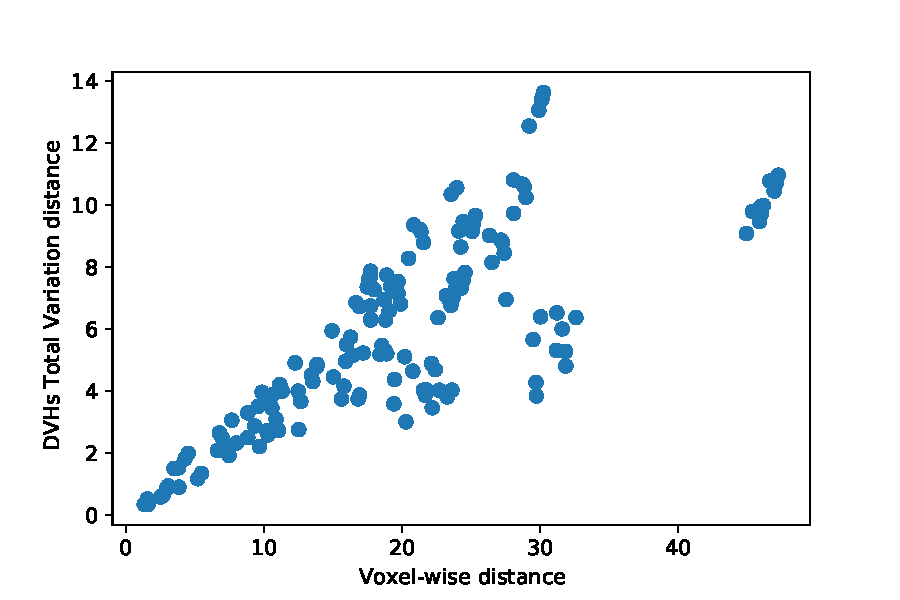
\includegraphics[width=0.49\textwidth]{dose_distances_figures/TotalVariation-Voxelwise.pdf}		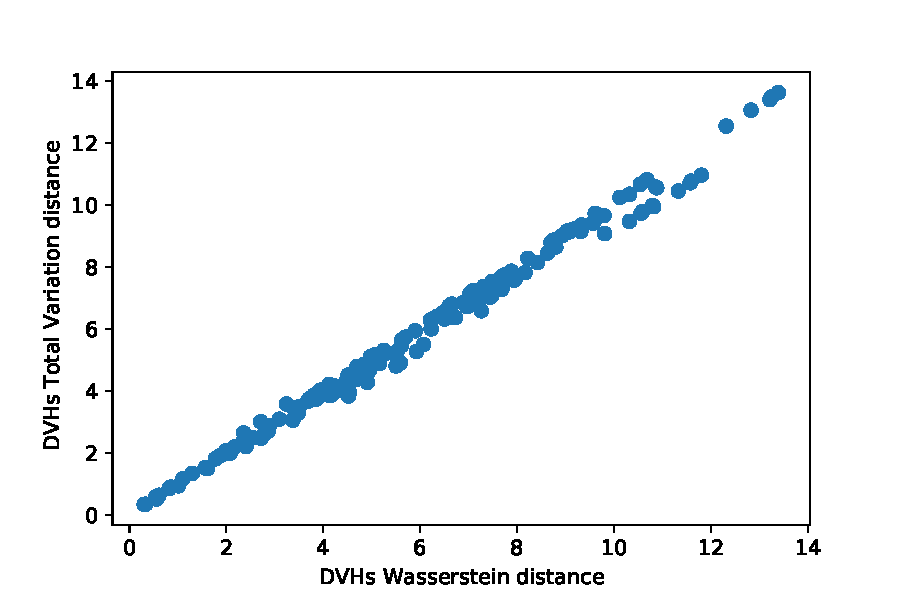
\includegraphics[width=0.49\textwidth]{dose_distances_figures/TotalVariation-Wasserstein.pdf}
%	\subfloat[\label{fig:TotalVariation-Voxelwise} DVHs Total Variation vs Voxel-wise]{\hspace{.5\linewidth}}
%	\subfloat[\label{fig:TotalVariation-Wasserstein} Total Variation vs Wasserstein]{\hspace{.5\linewidth}}
%	\caption{Comparing Distances}
%\end{figure}

\paragraph{Comparing Total Variation and Voxel-wise}
%The bounding of the total variation DVH distance in terms of voxel-wise distance is clear on figure \ref{fig:TotalVariation-Voxelwise} (there is a linear upper bound to the scatter plot).
%However, we can remark that some pair of distances are closer in terms of DVH than we imagined using just the voxel-wise distance; hence proving the necessity to analyze further than just the voxel-wise comparison.

\paragraph{Comparing Total Variation and Wasserstein}
%We observe (on figure \ref{fig:TotalVariation-Wasserstein}) that the two DVH distances are almost perfectly proportional.
%This was expected as they are equivalent mathematically, we only swapped axis of integration in the total variation (hence, the small fluctuations).



\subsection{Discussion}
%In this article, a novel metric for comparing radiation doses is introduced.
%This metric has the advantage of being insensitive to dose changes in some regions if being compensated in another region, which was the intended goal.
%This metric can be useful in several applications, such as dose mimicking and early stopping time for fluence map optimization optimization.
%
%However, there are some limitations to this distance metric.
%One drawback is that it does not capture spatial distribution, which can be a problem in some cases.
%There may be some pathological examples where the DVHs are similar, but the clinical interpretation is different.
%Other factors, such as the distribution of the dose within the target area or the surrounding tissues, can also play a crucial role in determining the effectiveness of the treatment.
%For example, if two doses have the same amount of high dose, one spread in several small high dose regions, and the other having one large high dose region, then the DVH could look alike, while doctors will interpret the two doses differently.
%These types of edge cases are, however, extremely rare in practice.
%We still advise, for critical cases, to use the voxel invariant metric in conjunction with other techniques to obtain a comprehensive evaluation of radiation doses.
%
%When comparing two different doses, a large distance between them could indicate a significant difference in the intensity or frequency of the treatment, but this does not necessarily mean that one dose is better than the other.
%The effectiveness of a dose also depends on several other factors such as the individual patient's characteristics, medical history, and response to the treatment.
%Thus, simply looking at the distance between doses may not provide an accurate picture of which dose is superior or more effective in a particular case.
%It is essential to consider all relevant factors when evaluating the efficacy of a treatment dose.
%
%Overall, our dose comparison technique is a promising tool.
%While it has some limitations, it can be a valuable addition to the arsenal of techniques used by radiation oncologists and medical physicists to optimize treatment plans and improve patient outcomes.

\paragraph{Stop Criterion}
Defining a meaningful stopping criterion for the FMO optimization process is a critical challenge in the context of radiotherapy dose optimization.
While optimization in clinical practice is often guided by dosimetrists, who may stop optimizing when they are satisfied with the result, the need for full automation of the optimization process necessitates the establishment of a systematic and objective stopping criterion.
One possible approach to defining a stopping criterion is to compare the clinical effect of two doses.
This would provide a useful tool for comparing different solutions and determining the point at which the optimization process can be terminated.



%%%%%%%%%%%%%%%%%%%%%%%%%%%%%%%%%%%%%%%%%%%%%%%%%%%%%%%%%%%%%%%%%%%%%%%%
%                                                                      %
%   %%%%%%%%%%%%%%%%%%%%%%%%%%%%%%%%%%%%%%%%%%%%%%%%%%%%%%%%%%%%%%%%   %
%   %%%%%%%%%%%%%%%%%%%%%%%%%%%%%%%%%%%%%%%%%%%%%%%%%%%%%%%%%%%%%%%%   %
%   %%%%%%%%%%%%%%%%%%%%%%%%%%%%%%%%%%%%%%%%%%%%%%%%%%%%%%%%%%%%%%%%   %
%   %%%%%%%%%%%%%%%%%%%%%%%%%%%%%%%%%%%%%%%%%%%%%%%%%%%%%%%%%%%%%%%%   %
%                                                                      %
%%%%%%%%%%%%%%%%%%%%%%%%%%%%%%%%%%%%%%%%%%%%%%%%%%%%%%%%%%%%%%%%%%%%%%%%



\section{Network of Doses}
% Clinically Meaningful Dose Clustering for Radiotherapy
\subsection{Introduction}
%Radiotherapy is a prevalent intervention for treating cancer, utilizing ionizing radiation to eliminate malignant cells.
%Among the various radiotherapy approaches, intensity-modulated radiation therapy (IMRT) stands out as a technique that administers high radiation doses to the tumor while minimizing exposure to surrounding healthy tissues \cite{ReportIMRT2003}.
%Traditional IMRT strategies employ several beams, usually 5, 7, or 9, originating from different angles around the patient \cite{Bortfeld2009TheNO}.
%Each beam's intensity is modulated to optimize radiation dose delivery to the tumor while reducing healthy tissue exposure.
%This technique surpasses the efficacy of the 3D-conformal radiotherapy (3D-CRT) approach \cite{KOLE2012} \cite{PALMA2008} \cite{VERHEY1999}.
%The multi-leaf collimator (MLC), a computer-controlled device, shapes the radiation beam to match the tumor's contours, facilitating precise and efficient delivery of the therapy.
%
%The efficacy of a radiotherapy treatment plan is contingent upon the optimization procedure.
%Optimization encompasses multiple steps:
%The first step is the beam angles choice.
%Most of the time, equispaced angles is chosen, as they offer the greatest flexibility \cite{Bortfeld_2006}.
%The second step (on which we will focus our study) is the Fluence Map Optimization (FMO).
%It consist of actually calculating a two dimensional map of fluence power for each angle.
%The fluence maps need to be a compromise between contradicting constraints on the Principal Target Volume (PTV) and the Organs At Risks (OARs).
%The third ans final step is the leaf sequencing.
%This is where we convert the ideal fluence maps computed before into machine instructions.
%Modern leaf sequencing algorithm (in particular, "sliding window" algorithm) perform very well \cite{Iqbal2013} \cite{Nicolini2005}.
%In this paper, we assume this part of optimization can be done perfectly.
%
%FMO is a key step to guarantee the most favorable administration of radiation.
%Computer softwares performing the optimization process, are called Treatment Planning Systems (TPSs).
%The use of a TPS is necessary given the complexity of the mathematical inverse problem to solve for the FMO.
%TPSs typically incorporate the patient's anatomy, tumor/organs' location and size, and the radiation objectives defined by medical professionals.
%
%There have been multiple attempts to automate the process of treatment optimization in radiation therapy.
%Several studies have focused on dose prediction (\cite{McIntosh_2017} \cite{Nguyen_2019}).
%These approaches aim to predict the optimal radiation dose for patients. Another avenue explored is the application of Pareto frontier exploration, as discussed in \cite{Kuipers2023} and \cite{Ottosson_2010}.
%This approach aims to identify a set of treatment plans that represent a trade-off between conflicting objectives.
%Additionally, \cite{CristianCotrutz_2003} proposed a method for directly extracting leaf movements from patient data.
%Despite these efforts, these automated approaches have not yet been adopted in clinical practice due to various limitations.
%In this paper, we present a hybrid approach that combines manual and automatic treatment optimization.
%Our algorithm generates a shortlist of potential doses, and the final selection is made by a medical professional.
%This approach aims to leverage the advantages of automation while incorporating the expertise and judgment of a doctor to ensure clinically usable treatment plans.


\subsection{Radiotherapy}
%This section provides a comprehensive description of the overarching framework encompassing the general setup of radiotherapy, elucidating the seamless integration of its various components within the clinical workflow.

\paragraph{Dose Optimization Inputs}
%The initial phase of the optimization process involves the generation of a virtual representation of the patient's anatomy using medical imaging technologies such as CT or MRI scans.
%This model is subsequently exploited to identify the tumor's size and location and delineate the adjacent healthy tissues that require protection from radiation exposure.
%The subsequent step is to establish the requisite radiation dose for effective treatment, with physicians typically prescribing dose-volume objectives (e.g., 95\% of Principal Target Volume or PTV should receive a minimum of 76Gy).
%The dose is determined based on factors such as tumor size, location, and type, as well as the patient's medical history and general well-being.
%These steps are undertaken by medical professionals.

\paragraph{Dose Simulation}
%In the radiation therapy optimization process, the next step involves computing the dose on the patient's volume by simulating one multi-leaf collimator (MLC) parametrization on the patient's body using medical imaging data.
%The computed dose is a map from the three-dimensional volume of the patient's body to a positive number of Grays, which is the unit used to measure the absorbed radiation energy.
%In practice, a discrete version of the dose is used, where the dose is calculated for each voxel of the patient's body.
%The influence of rays is mathematically modeled as a linear function of the transmitted energy within the radiation therapy optimization process.

\paragraph{Dose-Volume Histograms}
%Doctors have delineated the various relevant structures in the patient's anatomy to allow calculation of the dose-volume histogram (DVH) for each structure based on a given dose.
%The dose-volume objectives are then represented as points on the DVH that should be maintained either above (in case of minimum dose constraints) or below (in case of maximum dose constraints).

\paragraph{Evaluation of Doses}
%Doctors evaluate the quality of a dose using several criteria.
%First, they examine the 3D distribution of the dose on the patient's body, looking at the inter-structure distribution as well as the presence, number, and location of hot spots.
%Second, they analyze the DVH to determine if the curves match the predefined DVH objectives.
%This evaluation step is critical for ensuring that the surrounding healthy tissues are spared from unnecessary radiation exposure.
%By optimizing the treatment plan and verifying the quality of the dose, doctors can ensure the best possible outcome for the patient.


\subsection{Methods}
%The assurance of accuracy and efficacy in radiation therapy necessitates the implementation of robust dose optimization process.
%This is achieved after the optimization of an inverse problem \cite{Webb2003}; our specific implementation is described below.

\subsubsection{Radiotherapy Dose Optimization}

\paragraph{Simulation \& Approximation}
%The optimization process involved finding the optimal values for the bixels, denoted as $\textbf{b}$, while considering the dose distribution voxel-wise $\textbf{d}$ calculated based on the precomputed dose-influence matrix $\textbf{L}$, which relates bixels to the corresponding voxels.
%Here, we make the assumption that bixels activation and dose deposition are linearly linked.
%This assumption is very commonly used. %add citation?

\paragraph{Physical Limitations}
%It is important to note that due to the physical constraints of radiation therapy, it is not possible to have negative energy rays.
%Consequently, each bixel value should be non-negative ($b \geq 0 \quad \forall b \in \textbf{b}$).
%To ensure positive bixel values in practice, we applied an absolute value operation, computing $\textbf{d}=\textbf{L}\abs{\textbf{b}}$, where $\abs{\textbf{b}}$ represents the element-wise absolute value of $\textbf{b}$.

\paragraph{Mathematical Objective Function}
%In order to capture the diverse dose goals specified within the TG-119 data-set \cite{AAPM-TG119}, we designed a cost function that incorporates multiple objectives.
%The cost function employed in our study is a weighted sum of multiple objective functions, with each objective corresponding to a specific dose goal.
%The construction of the cost function is defined as follows, using a square over/under-dose penalty function for each objective:
%$$f(\textbf{d}) = \sum_{o \in \mathcal{O}} w_o f_o(\textbf{d})$$
%$$f_o(\textbf{d}) = \sum_{d \in \textbf{d}\left[ o_s \right]}(d - o_d)_+^2 \text{ if $o$ is a maximal dose-volume constraint}$$
%$$f_o(\textbf{d}) = \sum_{d \in \textbf{d}\left[ o_s \right]}(o_d - d)_+^2 \text{ if $o$ is a minimal dose-volume constraint}$$
%with:
%\begin{itemize}
%	\item $\textbf{d}$ the voxel-wise dose; $\textbf{d} \left[s\right]$ the dose on voxels of the structure $s$.
%	\item $\mathcal{O}$ the set of objectives (dose-volume goals)
%	\item $w_o$ is the weight of the objective $o \in \mathcal{O}$ (ranges typically between 0 and 100)
%	\item $o_s$, $o_d$ \& $o_v$ respectively the structure, dose and volume goals of $o \in \mathcal{O}$ (e.g.: $o_s$: PTV; $o_d$: 80Gy; $o_v$: 95\%)
%\end{itemize}
%The final function to optimize is $g(\textbf{b}) = f(\textbf{L}\abs{\textbf{b}})$.

\paragraph{MLC Fluence Discretization}
%We approximated the fluence of each beam using bixels.
%Bixels (\textbf{be}am-\textbf{el}ement) is a discrete element of the radiation beam that can be individually controlled to achieve spatially varying intensity levels.
%In our study, the width of these bixels was set to 5mm, corresponding to the width of leafs of the commonly used multi-leaf collimator.

\paragraph{Bixels Smoothness}
%To promote smoothness and consistency in the distribution of bixel values, we introduced a regularization term in our optimization.
%This penalty term that penalizes variations between neighboring bixels.
%Specifically, a square penalty was applied to the differences between bixel values and their neighboring counterparts.

\paragraph{Convexity}
%The cost function employed in our study is constructed to be convex by design, ensuring desirable mathematical properties for optimization.
%As a result, regardless of the specific set of weights assigned to the objectives, minimizing this cost function is expected to consistently converge to the same optimal radiotherapy plan.

\paragraph{Multiple Plans Generation}
%To generate diverse treatment doses for a given patient case and set of constraints, we employed a strategy of optimizing the cost function with different weight assignments for each constraint.
%Varying the weights associated with individual dose goals is how dosimetrists are now guiding optimization engines toward the best (clinically acceptable) solution.
%Playing with these weights allows to explore different trade-offs and prioritize certain aspects of the treatment plan over others.

\paragraph{Optimizer}
%The optimization of the main objective function was performed using the open-source optimizer L-BFGS (Limited-memory Broyden-Fletcher-Goldfarb-Shanno).
%This optimizer has been demonstrated to exhibit superior performance compared to other open-source optimizer available \cite{dubois2023}.

\subsubsection{Data}
\paragraph{(Phantom) Patient}
%The evaluation of our proposed method for clustering radiation doses was conducted using the TG-119 Prostate case \cite{AAPM-TG119}, which is a well-established benchmark data-set commonly employed for assessing the quality of radiation therapy plans.
%The TG-119 data-set encompasses predefined dose goals, which were utilized in the formulation of our cost function.

\paragraph{Dose normalization}
%We normalized the doses according to the "D50" normalization method, which is a common practice in the field of radiation therapy.
%It consists in normalizing the dose such that the median dose of the PTV is equal to the prescription dose.

\subsubsection{Dose Clustering Techniques}
\paragraph{Dose Distance}
%To cluster the doses, we first need to define a distance between them.
%We used the Euclidean distance between the voxel-wise doses.
%We defined the weight of the edge between two doses as the inverse of the distance between them
%(since we want to maximize the weight of the edges between similar doses).
%Defining the weight of the edge as the inverse of the distance between the doses is quite standard in the field of graph theory \cite{Maleika2020} \cite{Li2018}.

\paragraph{Community Detection}
\label{clustering_evaluation}
%We used the Louvain's method for community detection to cluster the doses.
%This method is a greedy optimization method that maximizes the modularity of the graph.
%The modularity of a graph is a measure of the quality of the partition of the graph into communities.
%We used the implementation of the Louvain's method in the python library networkx.

\paragraph{Evaluating Communities Split}
%Evaluation of clustering quality was performed using dose-volume histograms (DVH) obtained from different doses.
%The mean and standard deviation of the DVH were computed for each cluster versus the entire data-set:
%
%We conducted an analysis on the relative volume doses for the four distinct structures.
%A total of 101 dose values were sampled for each structure, with volume ranging from 0\% to 100\% equally spaced).
%These values were aggregated into a single vector, resulting in a vector length of 404 for each dose.
%
%To assess the variability within these dose vectors, we calculated the standard deviation for the 404 elements of each vector.
%This statistical measure provides insight into the dispersion of the dose values within a given structure.
%By averaging the obtained standard deviations, we derived a scalar metric that quantifies the degree of separation among a group of doses.


\subsection{Results}
\subsubsection{Doses Network}
\paragraph{Graph Plots}
%In figure \ref{fig:graph}, each node represents a dose.
%The communities are attributed using Louvain method and are identified by colors.
%Since the graph is clearly not planar, we choose to plot it in a circular layout (fig. \ref{fig:graph-circular}) and in a spring layout (fig. \ref{fig:graph-spring}).
%\begin{figure}
%	\centering
%	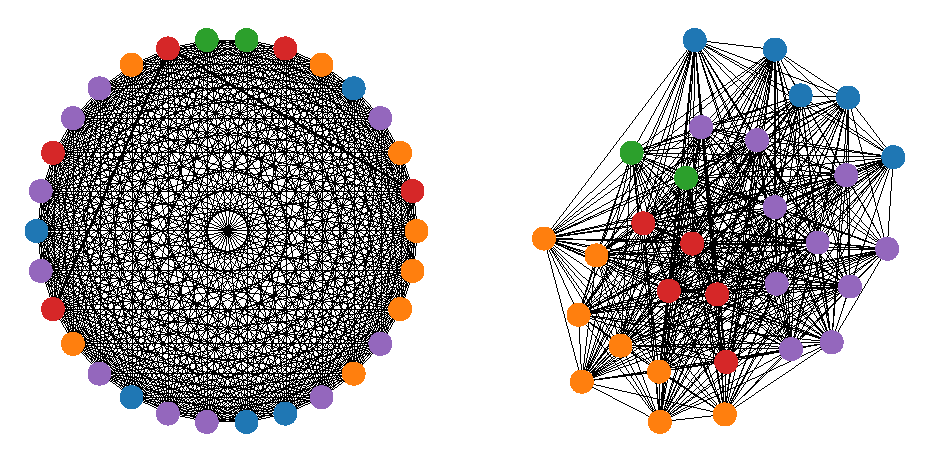
\includegraphics[width=0.40\textwidth]{dose_clustering_figures/graph.pdf}
%	\includegraphics[width=0.59\textwidth]{dose_clustering_figures/graph_bis.pdf}
%	\subfloat[\label{fig:graph-circular} (Circular Layout)]{\hspace{.5\linewidth}}
%	\subfloat[\label{fig:graph-spring} (Spring Layout)]{\hspace{.5\linewidth}}
%	\caption{
%		Plot of the Network\\
%		edges width $\propto$ edge weight $\propto$ $\nicefrac{\text{1}}{\text{distance}}$\\
%		node's color reflects community attribution
%	}
%	\label{fig:graph}
%\end{figure}

%In order to obtain a more precise understanding of the edge weights in the network, one can refer to the adjacency matrix of the edge weights, as depicted in Figure \ref{fig:adjacency}.
%\begin{figure}
%	\centering
%	\includegraphics[width=0.65\textwidth]{dose_clustering_figures/weight_adjacency_matrix.pdf}
%	\caption{Weight Adjacency Matrix of the Network}
%	\label{fig:adjacency}
%\end{figure}

\paragraph{DVH Plot}
%Figure \ref{fig:dvh} illustrates the Dose-Volume Histograms (DVHs), with the colors of the plots corresponding to the communities identified in the network analysis.
%To ensure clarity and prevent confusion, each structure is presented on a separate plot.
%Notably, our observations align with expectations, as doses assigned to nodes within the same community (indicated by the same color) exhibit nearly overlapping DVHs.
%\begin{figure}
%	\centering
%	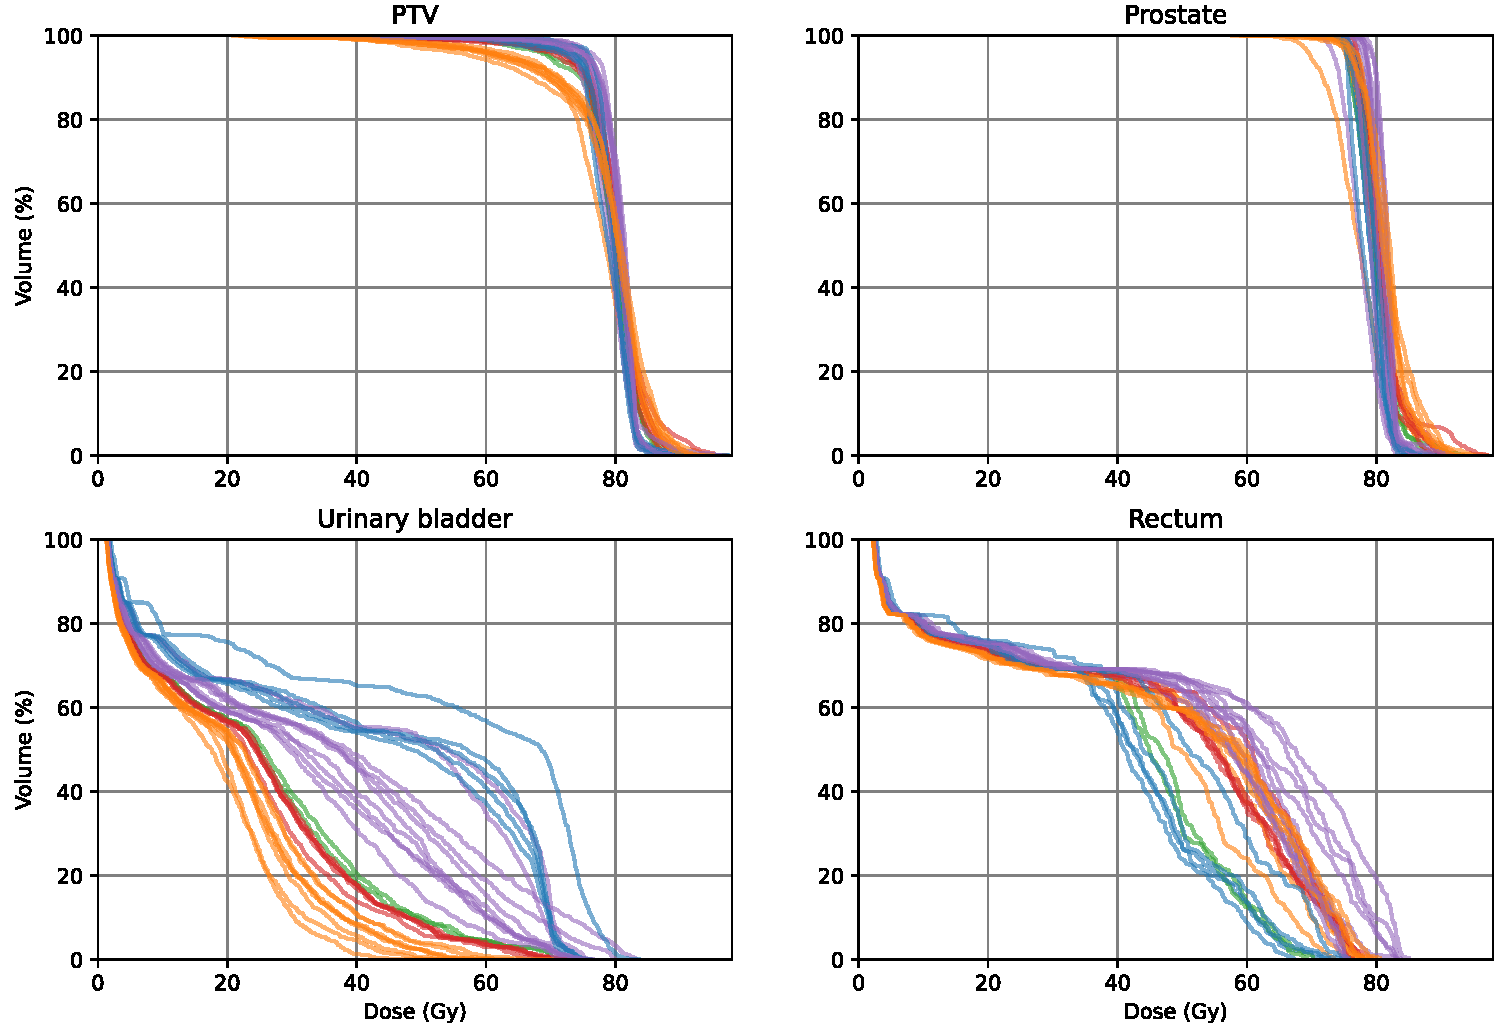
\includegraphics[width=\textwidth]{dose_clustering_figures/dvh.pdf}
%	\caption{Dose-Volume Histogram}
%	\label{fig:dvh}
%\end{figure}

%The visualization of DVHs provides valuable insights into the distribution of doses received by different structures.
%The close correspondence between dose patterns and community assignment underscores the potential of network analysis in uncovering meaningful patterns within radiation therapy data.
%By associating the colors of the DVH plots with the communities identified in the network, we gain a deeper understanding of the relationship between dose assignments and structural characteristics.
%This analysis further supports the notion that nodes (doses) within the same community share similar profiles, suggesting they could be merged, as they will likely have the same clinical effect.

\subsubsection{Dose Clustering Evaluation}
%As explained in \ref{clustering_evaluation}, we use the mean standard deviation of doses at 101 equispaced values of volume to obtain a scalar value of how far apart are a set of doses; see table \ref{table:cluster_std} for results.
%
%\begin{table}
%	\centering
%	\begin{tabular}{|l|c|c|}
%		\hline
%		Set & Set Size & Mean Standard Deviation \\
%		\hline
%		Cluster 1 \textcolor{plt-blue}  {\textbf{(blue)}}   & 4 & 2.0542 \\
%		Cluster 2 \textcolor{plt-orange}{\textbf{(orange)}} & 5 & 0.4049 \\
%		Cluster 3 \textcolor{plt-green} {\textbf{(green)}}  & 2 & 0.3618 \\
%		Cluster 4 \textcolor{plt-red}   {\textbf{(red)}}    & 2 & 0.4218 \\
%		Cluster 5 \textcolor{plt-purple}{\textbf{(purple)}} & 3 & 0.9702 \\
%		Cluster 6 \textcolor{plt-brown} {\textbf{(brown)}}  & 3 & 1.2418 \\
%		\textit{All} & \textit{19} & \textit{3.5122} \\
%		\hline
%	\end{tabular}
%	\caption{Clustering Quality}
%	\label{table:cluster_std}
%\end{table}
%
%The mean standard deviation of the clusters, with values of 2.0542, 0.4049, 0.3618, 0.4218, 0.9702, and 1.2418, averaging at 0.9091, is significantly lower (nearly 4 times lower) compared to the mean standard deviation of the full network, which is 3.5122 (see table \ref{table:cluster_std}).
%This notable reduction in standard deviation yells quantitatively that our clustering approach has favorable results.
%This quantitative assessment is further supported by qualitative results, as illustrated in Figure \ref{fig:dvh}, which demonstrates the meaningfulness and relevance of the dose clusters in characterizing radiation dose distributions.
%Our proposed clustering approach demonstrates strong performance in both qualitative and quantitative evaluations.

\subsection{Discussion}
%The ability to regroup doses into communities provides a valuable insights to understand clinical practices.
%An additional potential application of this technique is the utilization of dose clusters as a similarity measure for early stopping optimization purposes.
%Specifically, if the dose distribution exhibits similarities to the previous $n$ doses, it may serve as an indicator to halt the ongoing optimization process.
%
%However, the clustering of doses is a challenging task, as the dose space is high dimensional and the dose distribution is not smooth.
%The results presented here can not yet be used in clinical practice, they are promising and should be further investigated.

\subsection{Conclusion}
%In conclusion, this study has introduced a novel approach for clustering doses into communities based on their dose distributions, demonstrating the meaningfulness of such clustering both quantitatively and qualitatively.
%This suggests that doses belonging to the same cluster are likely to have indistinguishable clinical effects.
%
%The proposed clustering technique holds several potential applications.
%Firstly, it can be integrated into Fluence Map Optimization (FMO) to facilitate early stopping of the optimization process when the last few updates remain within the same cluster, providing efficiency gains.
%Secondly, if extended to clustering doses from different patients, it could enable the analysis of clinical center practices, offering insights into variations in treatment outcomes among centers for specific anatomies.
%
%Furthermore, this clustering approach has the potential to streamline the validation process between dosimetrists and physicists.
%Currently, multiple treatment plans are submitted for validation, leading to a cumbersome selection process for the physicist.
%However, by clustering the optimized doses with different weight parameters for constraints, the number of options can be reduced, resulting in a more efficient decision-making process and potentially reducing the personnel required in the dosimetry department.
%
%As further research and validation efforts are undertaken, this innovative approach holds considerable promise for enhancing treatment planning processes and, ultimately, improving patient outcomes.



%%%%%%%%%%%%%%%%%%%%%%%%%%%%%%%%%%%%%%%%%%%%%%%%%%%%%%%%%%%%%%%%%%%%%%%%
%                                                                      %
%   %%%%%%%%%%%%%%%%%%%%%%%%%%%%%%%%%%%%%%%%%%%%%%%%%%%%%%%%%%%%%%%%   %
%   %%%%%%%%%%%%%%%%%%%%%%%%%%%%%%%%%%%%%%%%%%%%%%%%%%%%%%%%%%%%%%%%   %
%   %%%%%%%%%%%%%%%%%%%%%%%%%%%%%%%%%%%%%%%%%%%%%%%%%%%%%%%%%%%%%%%%   %
%   %%%%%%%%%%%%%%%%%%%%%%%%%%%%%%%%%%%%%%%%%%%%%%%%%%%%%%%%%%%%%%%%   %
%                                                                      %
%%%%%%%%%%%%%%%%%%%%%%%%%%%%%%%%%%%%%%%%%%%%%%%%%%%%%%%%%%%%%%%%%%%%%%%%


\section[Novel Dosimetry Automation Approach with Graph Theory]{A Novel Framework for Multi-Objective Optimization and Robust Plan Selection Using Graph Theory (ESTRO 2024)}
% many-clicks to few-clicks solution, but goal is one-click
% N-clicks to 2/3-clicks solution, but goal is 1-click

% Poster:
% https://github.com/pauldubois98/ESTRO2024/blob/main/poster-dose_clustering.pdf
% Abstract:
% https://docs.google.com/document/d/1c5GWgAm6TgaTgsQqJVnz9GaSjIlCgfAideT8Rsz4frM/edit?usp=sharing
